\newpage
\hypertarget{allCards tex}{}
\subsection{Text new rule}
\texHeader

Create a new rule in the appropriate folder called \texttt{AllOtherCardsRule}

% Object variables (pre condition)
Lets think about what needs to be done: this will only be called if there is a fourth partition that can't be matched. That means we already know/have Box, an
initial partition partition0, and a lst partition, partitionN.  Create each of these black object variables, then create one more for our fourth partition.
name it partitionNN. We don't need a correspondence or target becazse.. (we're just accomodating this extra one.) no need to set up a NEW target - we're working exclusively within box to include this extra card in the pattern and assuming dictionary already exists. By
consequence, we don't need to set up a NEW correspondence to Dictionary, just box <- allOtherCards : AllOtherCards -> dictionary

% Linkage
We'll need to connect partitionN to partitionNN via the \texttt{next} attribute, and connect partitionN to partition0 via a \texttt{previous} reference

% Attributes % constraint
Knowing that our final matched partition will be of index 2 or greater, establish a binding operator of partitionN.index >= 2. This will ensure NN is our n+1th
addition. contrain this in the final scope by adding: add(partitionN.index, 1, partitionNN). Syntax is: it should be explained that the syntax for this is
x+y=z, where add(x,y,z).

What are some other ways you could have constructed this same rule? i.e., does each reference you just declared HAVE to be in their current position?

Your completed rule should now resemble Fig.~\ref{}

\begin{figure}[htbp]
\begin{center}
  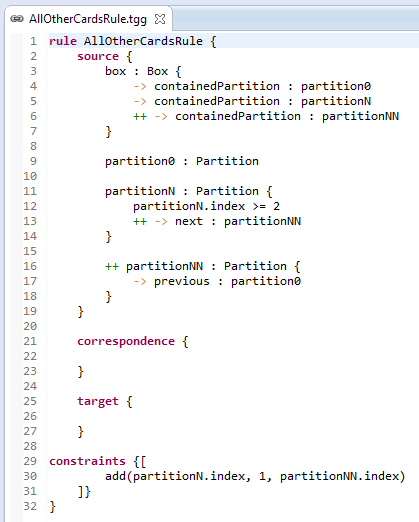
\includegraphics[width=0.7\textwidth]{eclipse_allOtherCardsRule}
  \caption{All Other Cards Rule Complete}
  \label{fig:allOtherCardsRule}
\end{center}
\end{figure}

Alles gut! Save and build. Make sure no errors in the generated files. (then move on)
